\documentclass[border=6pt]{standalone}
\usepackage{tikz}
\usetikzlibrary{arrows.meta,positioning,calc,shapes.geometric,fit,backgrounds,patterns,matrix,decorations.pathreplacing}
\begin{document}
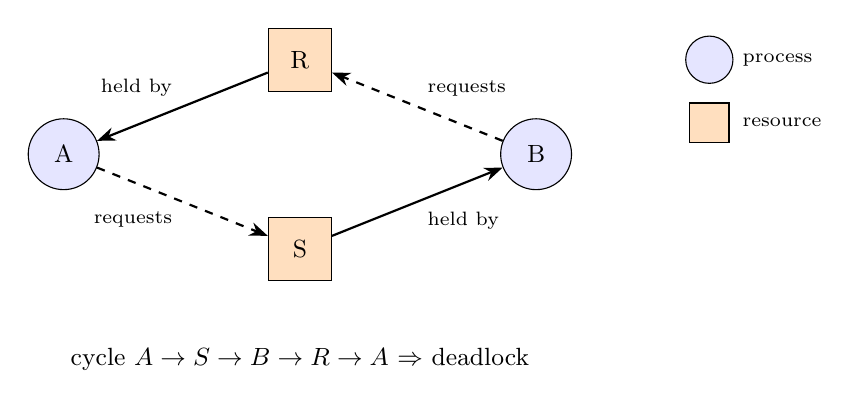
\begin{tikzpicture}[>=Stealth,font=\small]
\tikzstyle{pr}=[circle,draw,minimum size=0.9cm,fill=blue!10]
\tikzstyle{rs}=[rectangle,draw,minimum size=0.8cm,fill=orange!25]
\node[pr] (A) at (0,0) {A}; \node[rs] (R) at (3,1.2) {R}; \node[pr] (B) at (6,0) {B}; \node[rs] (S) at (3,-1.2) {S};
\draw[->,thick] (R) -- node[above left,font=\scriptsize]{held by} (A);
\draw[->,thick,dashed] (A) -- node[below left,font=\scriptsize]{requests} (S);
\draw[->,thick] (S) -- node[below right,font=\scriptsize]{held by} (B);
\draw[->,thick,dashed] (B) -- node[above right,font=\scriptsize]{requests} (R);
\node[font=\small,align=center] at (3,-2.6) {cycle $A\to S\to B\to R\to A$ $\Rightarrow$ deadlock};
\node[pr,fill=blue!10,minimum size=0.6cm] at (8.2,1.2) {}; \node[font=\scriptsize,right] at (8.5,1.2) {process};
\node[rs,minimum size=0.5cm] at (8.2,0.4) {}; \node[font=\scriptsize,right] at (8.5,0.4) {resource};
\end{tikzpicture}
\end{document}
